\documentclass[10pt,conference,letterpaper]{IEEEtran}
\usepackage{graphicx}
\usepackage{subfigure}
\begin{document}
\section{experiment}

\begin{figure}[!htbp]
\centering
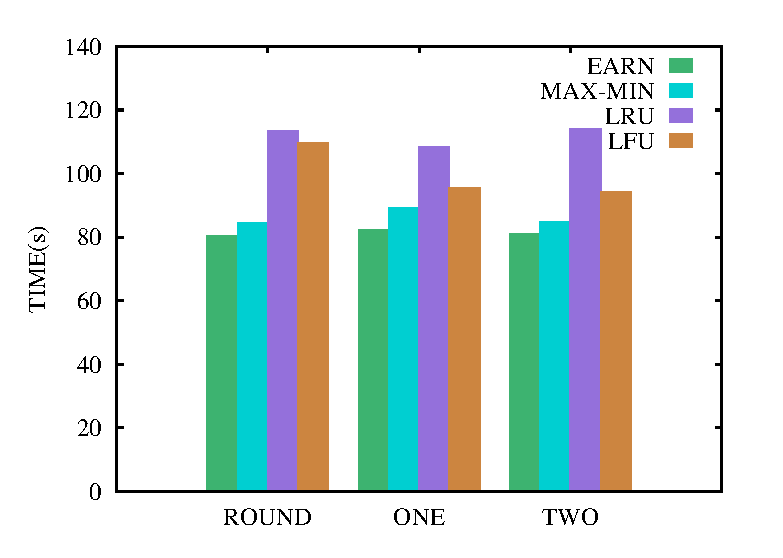
\includegraphics[scale=0.4]{figures/scan444_time.eps}
\caption{Access Time. Three files are equal in size (40GB).}
\label{fig:time_444}
\end{figure}

\begin{figure}[!htbp]
\centering
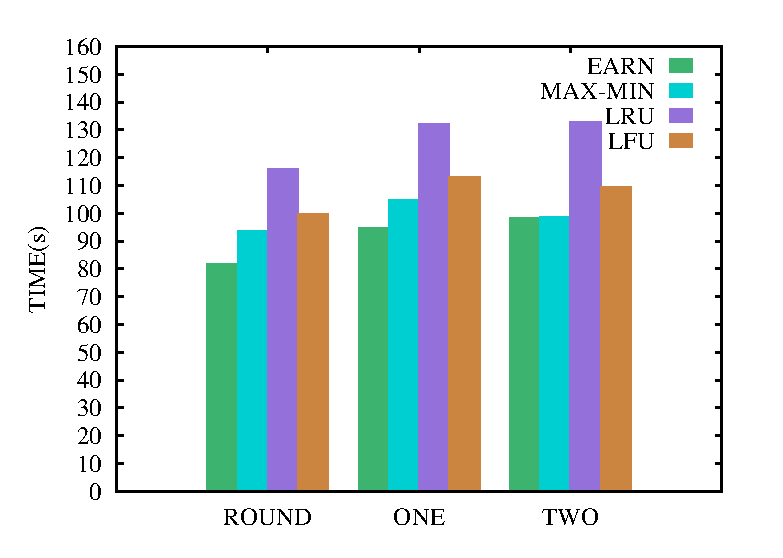
\includegraphics[scale=0.4]{figures/scan741_time.eps}
\caption{Access Time. The size of files is 70GB, 40GB and 10GB respectively.}
\label{fig:time_741}
\end{figure}

\begin{figure}[!htbp]
\centering
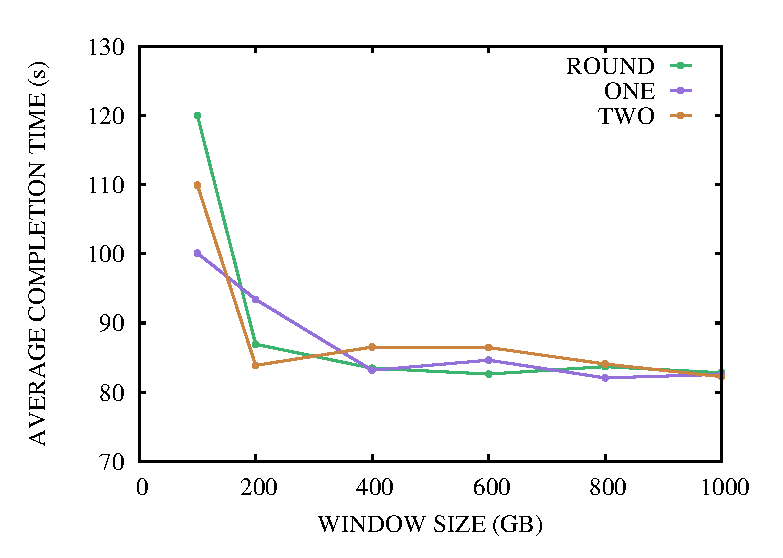
\includegraphics[scale=0.4]{figures/window_size_time.eps}
\caption{Access Time. Each with different window size.}
\label{fig:time_windowsize}
\end{figure}


\begin{figure}[!htbp]
    \subfigure[ROUND]{
    		\begin{minipage}[b]{0.25\linewidth}
    		\centering
    		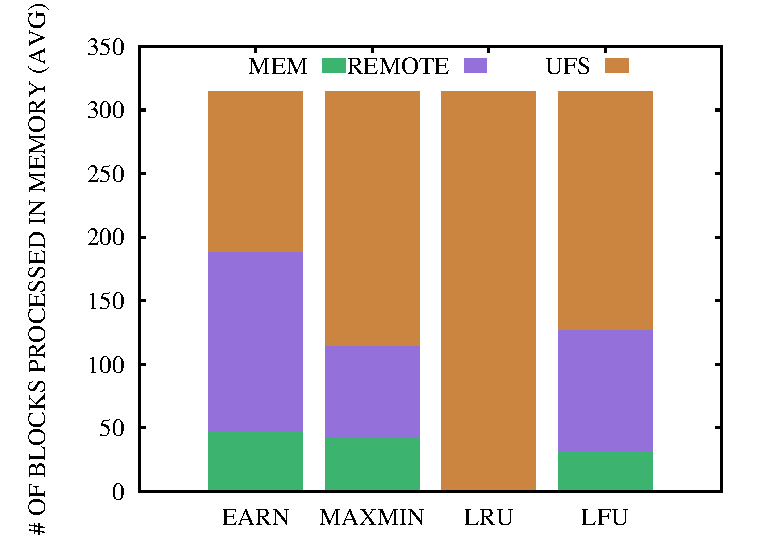
\includegraphics[scale=0.2]{figures/block_count_avg_round.eps}
    		\end{minipage}
    }
    \subfigure[ONE]{
        \begin{minipage}[b]{0.25\linewidth}
        \centering
        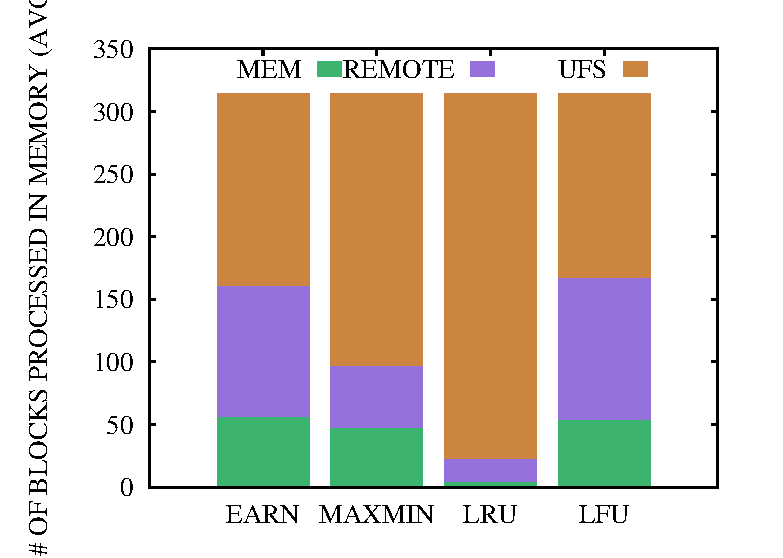
\includegraphics[scale=0.2]{figures/block_count_avg_one.eps}
        \end{minipage}
    }
    \subfigure[TWO]{
        \begin{minipage}[b]{0.25\linewidth}
        \centering
        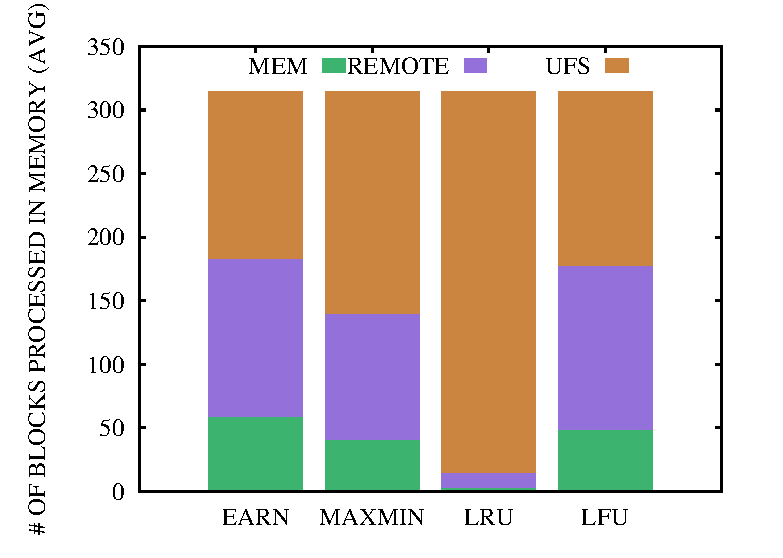
\includegraphics[scale=0.2]{figures/block_count_avg_two.eps}
        \end{minipage}
    }
    \caption{Distribution of blocks accessed in memory, remote memory and under file system.}
    \label{fig:block_count}
\end{figure}


\begin{figure}[!htbp]
    \subfigure[EARN]{
    		\begin{minipage}[b]{0.45\linewidth}
    		\centering
    		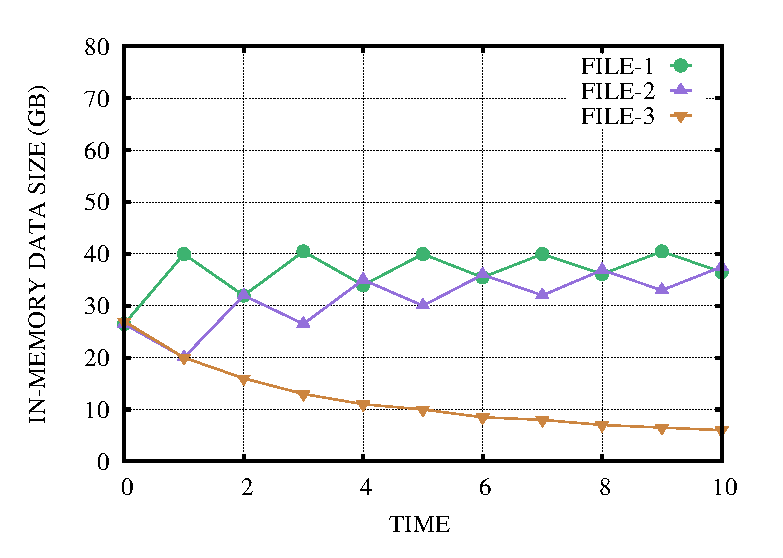
\includegraphics[scale=0.34]{figures/3-1-earn-1000-ds.eps}
    		\end{minipage}
    }
    \subfigure[MAXMIN]{
        \begin{minipage}[b]{0.45\linewidth}
        \centering
        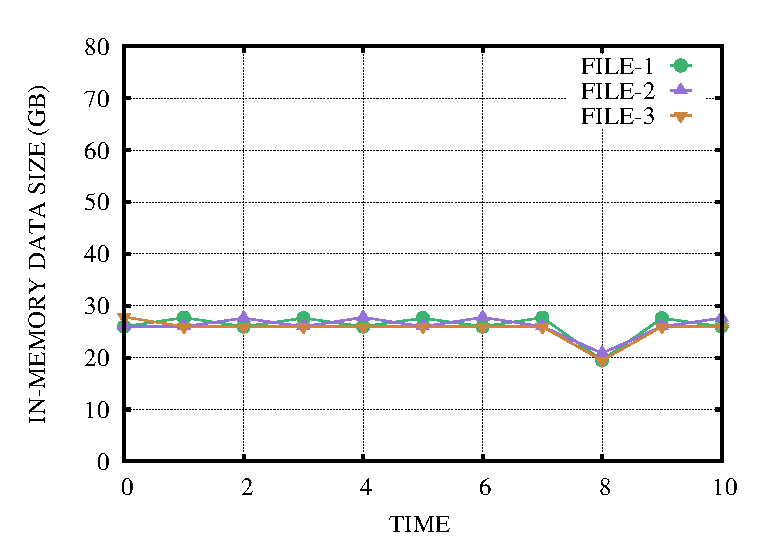
\includegraphics[scale=0.34]{figures/3-1-maxmin-1000-ds.eps}
        \end{minipage}
    }
    \caption{In-memory data size of each file after File-3 stops been visited.}
    \label{fig:3-1}
\end{figure}


\begin{figure}[!htbp]
    \subfigure[EARN]{
    		\begin{minipage}[b]{0.45\linewidth}
    		\centering
    		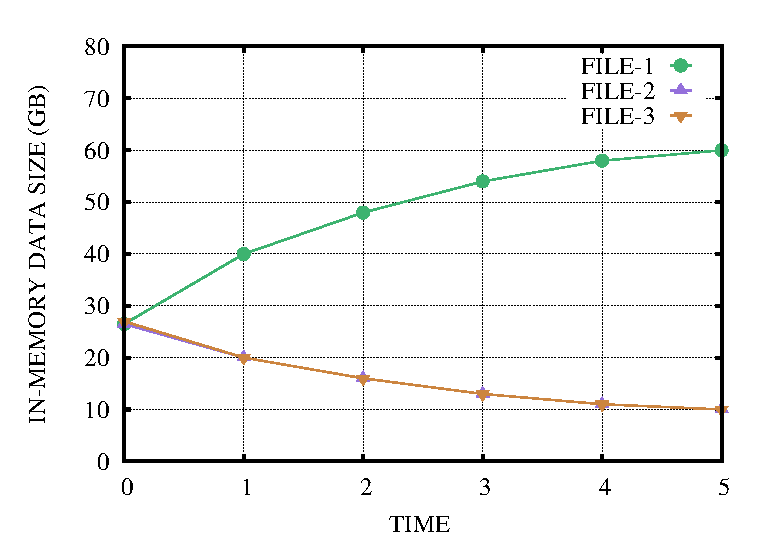
\includegraphics[scale=0.34]{figures/3-2-earn-1000-ds.eps}
    		\end{minipage}
    }
    \subfigure[MAXMIN]{
        \begin{minipage}[b]{0.45\linewidth}
        \centering
        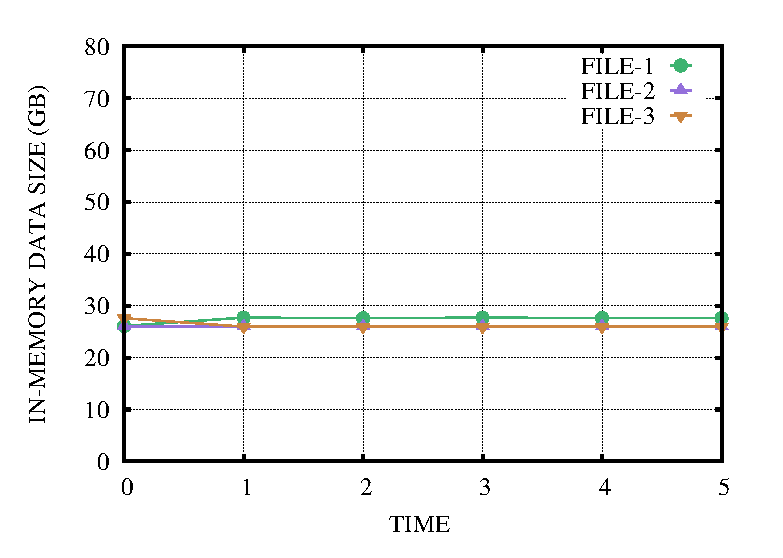
\includegraphics[scale=0.34]{figures/3-2-maxmin-1000-ds.eps}
        \end{minipage}
    }
    \caption{In-memory data size of each file after File-3 and File-2 stop been visited.}
    \label{fig:3-2}
\end{figure}

\end{document}